%mark = star, diamond, square, otimes
%\documentclass{article}
%\usepackage{pgfplots}
%\usepackage[justification=centering]{caption}
%\pgfplotsset{compat=newest}
%\begin{document}
\begin{figure}
\centering

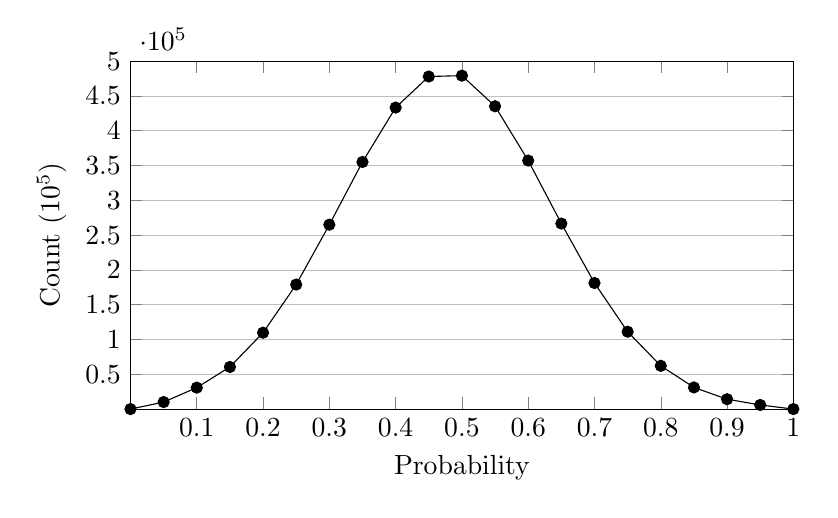
\begin{tikzpicture}
\begin{axis}[
 width=10cm,
   height=6cm,
    xlabel={Probability },
    ylabel={Count ($10^5$)},
    xmin=0, xmax=1.0,
    ymin=0, ymax=500000,
    xtick={.1,.2,.3,.4,.5,.6,.7,.8,.9,1.0},
    ytick={50000,100000,150000,200000,250000,300000,350000,400000,450000,500000},
    legend pos=north east,
    ymajorgrids=true,
    grid style={line width=.2pt,draw=gray!50},
]
 
\addplot[
    solid, every mark/.append style={solid, fill=black}, mark=*
    ]
    coordinates {
			(0,0)
			(0.05,10068)
			(0.1,30825)
			(0.15,60529)
			(0.2,109792)
			(0.25,178975)
			(0.3,265006)
			(0.35,355127)
			(0.4,433334)
			(0.45,477961)
			(0.5,479225)
			(0.55,435233)
			(0.6,357179)
			(0.65,266639)
			(0.7,181169)
			(0.75,111182)
			(0.8,62178)
			(0.85,31116)
			(0.9,14207)
			(0.95,5909)
			(1,0)
};
 
\end{axis}
\end{tikzpicture}
\caption{Probability Distribution for \emph{T40I10D100K} data set}
\label{result:t10}
\end{figure}
%\end{document}